
\begin{frame}
\frametitle{Paměťový subystém - Intel Nehalem}

{
\centering

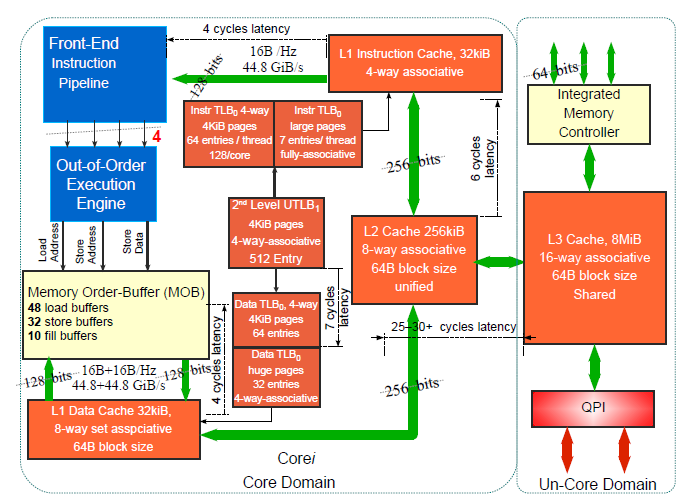
\includegraphics[width=0.80\linewidth]{common/arch/x86/mem-nehalem-lat.png}

}

\end{frame}

\begin{frame}
\frametitle{Stránkování na 64-bitových architekturách}

Plná 64-bitová délka fyzické adresy nemá (zatím) použití.
Aní 64-bitová virtuální adresa. Úrovně zpomalují běh.
Nejvyšší bity se nahrazují znaménkvým rozšířením.
Horní oblast operační systém, spodní pro aplikace.
Další optimalizace volitelné velké stránky -- huge pages.

{
\centering

\includegraphics[width=0.6\linewidth]{generated/memory/paging/paging-canonical-64-bit.pdf}

}
\end{frame}
